\documentclass{ltjarticle}

\usepackage{graphicx}
\usepackage{hyperref}
\usepackage{subcaption}
\usepackage{xcolor}
\usepackage{amssymb}
\usepackage{amsmath}
\usepackage{authblk}

\title{Computer Vision for Comparison and Display of Different Versions of Woodblock-printed Books and its Application to Bukan}

\author[1,3]{Thomas Leyh}
\author[2,3]{Asanobu Kitamoto}
\affil[1]{University of Freiburg}
\affil[2]{ROIS-DS Center for Open Data in the Humanities}
\affil[3]{National Institute of Informatics}

\date{July 7th, 2020}

\usepackage[backend=biber,style=alphabetic,sorting=nyt]{biblatex}
\addbibresource{references.bib}

\begin{document}

\maketitle

\section{Introduction}

In the Digital Humanitites, one of the basic goals is to make comparison possible. This allows for easier classification and enables search inside a dataset. On the one hand, there are numerous text-based methods along with large corpera of literary text. On the other hand, the emerge of large image datasets directly leads to methods from Computer Vision, skipping the necessarity of text transcriptions. This paper describes the technical development of this approach as well as its application to Bukan, a special type of Japanese woodblock printed books.

The authors have been approaching this problem in the past. \cite{kitamoto2018} proposed the concept of “differential reading” for visual comparison. Furthermore, \cite{hakim2019} proposed “visual named-entity recognition” for identifying family crests, using them for a page-by-page matching across different versions. This paper is a follow-up of these works and proposes a keypoint-based method for the page-by-page matching, additionally yielding an option for highlighting differences. 

\section{Dataset}

This work is mainly concerned with extracting information from a specific type of book: 武鑑---Bukan. These are historic Japanese books from the Edo period (1603-1868). Serving as \emph{unofficial} directories of Japanese bureaucrats, they include a wealth of information about regional characteristics such as persons, families and other key factors. See figure~\ref{fig:shuugyokubukan006} for an example. These books were created with woodblock-printing. Because the same woodblock has been reused for many versions of the book---sometimes with minor modifications---visual comparison can reveal which part of the woodblock was modified or has degraded.

\begin{figure}
    \centering
    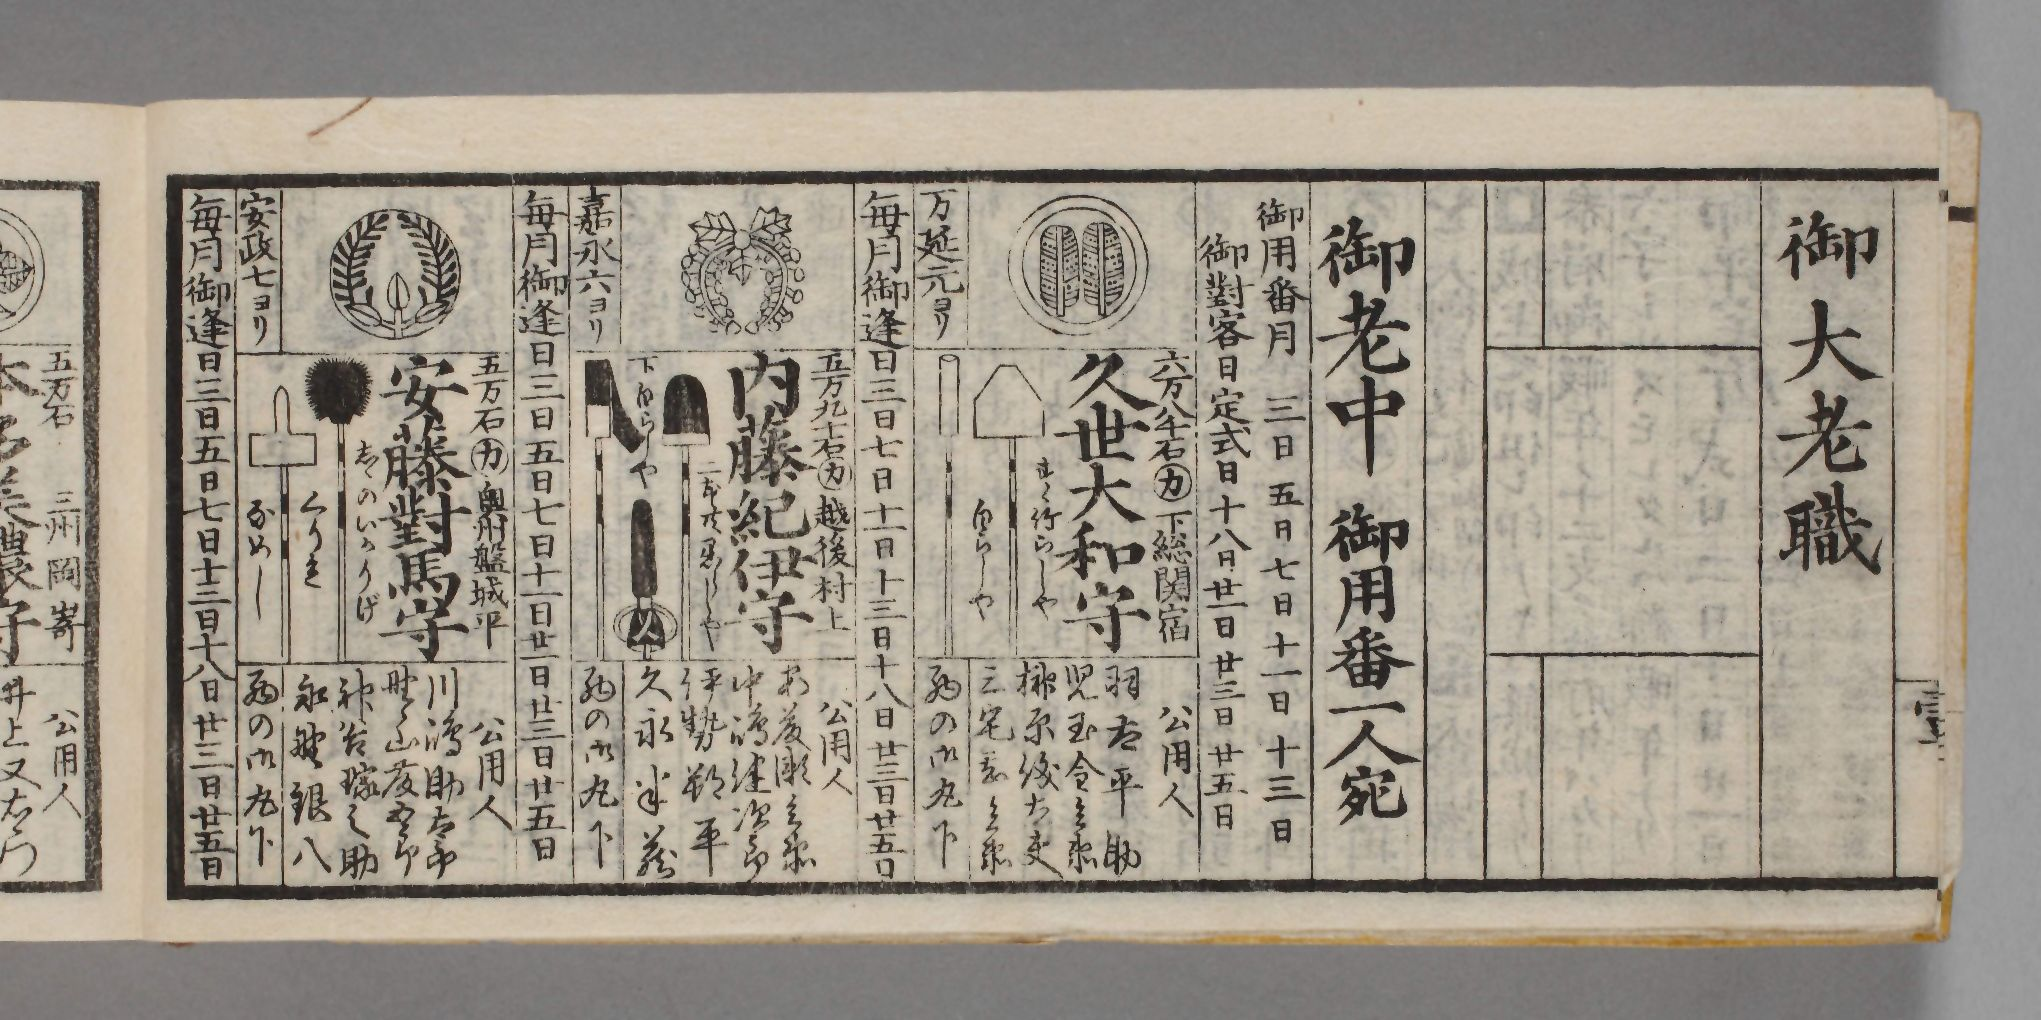
\includegraphics[width=\textwidth]{200019500_00006}
    \caption[Shūgyoku Bukan (袖玉武鑑), page 6]{Shūgyoku Bukan (袖玉武鑑) from 1861, page 6; showing names, descriptions, family crests and procession items. Especially interesting are the blank areas on the right, because in other edition they contain text.}
    \label{fig:shuugyokubukan006}
\end{figure}

ROIS-DS Center for Open Data in the Humanities and the National Institute of Japanese Literature are offering 381 of these Bukan as open data \cite{pmjt}. The original images have a width of $5616$ and height of $3744$ pixels. Under the assumption that this task (1) does not require this level of detail, (2) does not require information about color and (3) only compares the actual pages, not the surrounding area, basic image transformations are applied. All scans are resized by $25\%$, converted to grayscale and finally cropped, resulting in an image shape of $990 \times 660$ pixels. If there are two book pages per scan, they were additionally split at their horizontal center.

\section{Method}

Using an approach based on Computer Vision, two techniques were applied:

\begin{enumerate}
    \item \emph{Keypoint Detection and Matching} for finding the same features in different images.
    \item \emph{Projective Transformations} for comparing two different images regardless of their original orientation.
\end{enumerate}

We used the mature \emph{OpenCV} software library.\cite{opencv_library} 

\section{Results}

Integer finibus libero vestibulum quam aliquam, nec dictum neque lacinia. Suspendisse vulputate porta dictum. Duis ornare enim tortor, sit amet accumsan neque hendrerit non. Nunc auctor ipsum et ornare finibus. Proin maximus aliquam lobortis. Donec sed ullamcorper metus, vel posuere ex. Curabitur efficitur risus ante, vel auctor odio suscipit vulputate. Donec ut justo et lacus consectetur commodo eget sed tellus. Quisque rutrum, nunc sit amet euismod efficitur, dui nisi bibendum leo, interdum ultricies est lorem vitae tortor. Praesent lorem tortor, molestie a scelerisque ut, ornare vitae urna. Suspendisse faucibus sollicitudin dui vel pellentesque. Suspendisse potenti. Aenean sollicitudin placerat lacus nec tempor.

Nam mollis, eros nec fringilla ultrices, diam lorem tempus justo, consectetur commodo magna lorem in dui. Suspendisse laoreet nulla at convallis egestas. Maecenas ipsum nunc, ornare et nisi finibus, tempor facilisis eros. Pellentesque fermentum a dolor sit amet congue. Pellentesque consequat congue dictum. Donec leo velit, faucibus sit amet magna ut, pretium molestie velit. Aliquam lobortis commodo sodales. Nam posuere facilisis egestas. Nam libero nibh, lacinia a velit non, commodo maximus erat. Proin pellentesque massa eget diam faucibus molestie. Donec vel malesuada massa. Nam accumsan nibh nec leo imperdiet, sit amet sodales sapien varius.

Aenean bibendum quam est, id hendrerit nisl vulputate non. Phasellus dictum laoreet orci nec commodo. Vestibulum ante ipsum primis in faucibus orci luctus et ultrices posuere cubilia curae; Ut in sem tincidunt, varius nibh a, rutrum massa. Fusce pulvinar vel nibh a volutpat. Cras et lacinia dui. Ut varius auctor efficitur. Nullam egestas eleifend ante sed pellentesque. Proin eget lorem quis eros tincidunt tempor vel id tellus. Integer lobortis, magna molestie mollis consequat, libero dui sagittis eros, ac porttitor quam orci non lacus. Phasellus dignissim lacus nec interdum gravida. Sed ultricies arcu nec rhoncus porttitor. Mauris porttitor id neque posuere fringilla. Pellentesque non commodo elit. Vivamus eleifend odio ante, sed mollis ex porttitor eu. In accumsan arcu vel imperdiet ornare. Integer euismod, lectus a laoreet gravida, ante felis. 

% Computer vision-based approach consists of two steps as follows.

% \begin{enumerate}
%     \item \emph{Keypoint Detection and Matching} for finding the same features in different images.
%     \item \emph{Projective Transformations} for comparing two different images regardless of their original orientation.
% \end{enumerate}

% We used \emph{OpenCV} software library.\cite{opencv_library} to implement these steps. 

% \subsection{Keypoint Matching}
% \label{sec:keypoint-matching}

% T\emph{Keypoint Detection}\cite[Ch.4]{szeliski2010computer} is to find points of interest in an image that are most noticeable and give a unique description of the local area surrounding them.  Computer Vision research produced various kinds of keypoints, most prominently \emph{SIFT}.\cite{lowe2004sift} For evaluating the performance of these algorithms, 12 prints of the \emph{Shūchin Bukan} (袖珍武鑑) were manually annotated, in total around 1800 pages, holding information about the position of matching pages. 


% However, most of the time an identical page number corresponds to matching page content (e.g. page 10 of two prints was made using the same woodblock). To remove this bias, a potential matching of all possible page-keypoint combinations was computed while discarding matching pages where the number of matching keypoints was below a given threshold. The metric for evaluation is the value at the intersection of the precision and the recall curve. The following algorithms were evaluated:

% \begin{itemize}
%     \setlength\itemsep{0em}
%     \item ORB\cite{rublee2011orb}
%     \item AKAZE\cite{alcantarilla2011fast}
%     \item AKAZE without rotational invariance (UPRIGHT)
%     \item BRISK\cite{leutenegger2011brisk}
%     \item SIFT and SURF\cite{bay2006surf}, but these are not further considered since they are lacking performance on this task
% \end{itemize}

% \begin{figure}
%     \centering
%     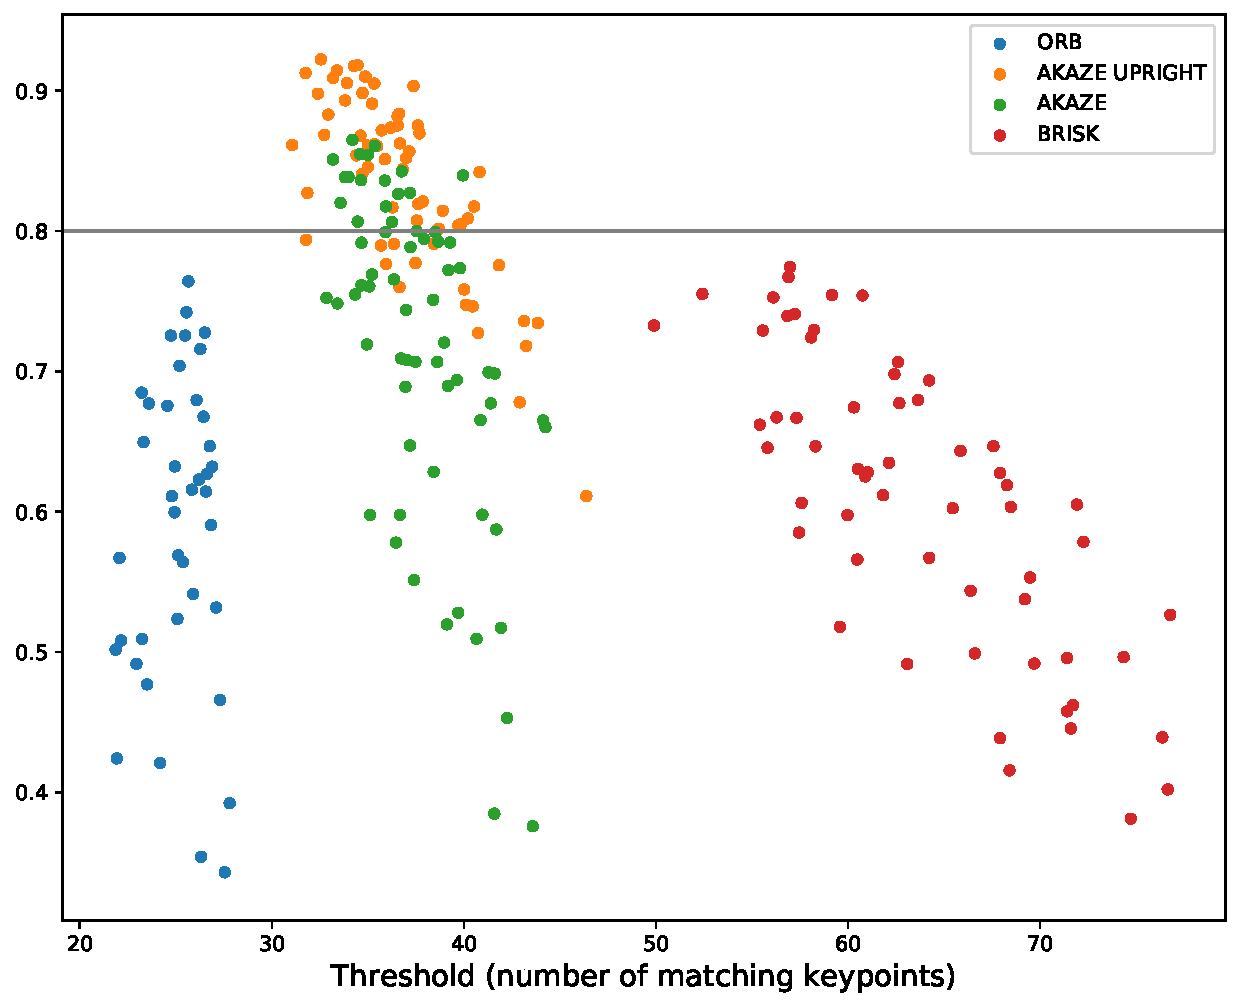
\includegraphics[width=\textwidth]{keypoint-evaluation.pdf}
%     \caption[Scatterplot of keypoint performance]{Scatterplot showing the positions of intersection of various precision-recall curves depending on the threshold of the number of matching keypoints. All points above the gray horizontal line at $0.8$ are considered “good enough” by the author. Even though this metric discards much information, there is a general tendency in favor of AKAZE UPRIGHT discernible.}
%     \label{fig:keypoint-evaluation}
% \end{figure}

% The results are presented in figure \ref{fig:keypoint-evaluation}. AKAZE UPRIGHT seems to have the best performance. Here, rotational invariance was explicitly \emph{not} included since the original images were scanned after cleanly aligning them on a table. This seems to bolster the keypoints' discriminative power. Nevertheless, the current results are far from satisfactory; from a performance standpoint as well as from the stability of the approach. Can we improve upon this by incorporating additional information?

% \subsection{Projective Transformations}
% \label{sec:projective-transformations}

% A Projective Transformation (or \emph{Homography}) is a matrix $\mathbf{H}$ for transforming homogeneous coordinates $\mathbf{H}\vec{x} = \vec{y}$. This not only allows linear transformations like translation and rotation but also perspective transformations. For finding such a transformation from matching keypoints, the heuristic \emph{Random Sample Consensus} (RANSAC) algorithm is used.\cite{fischler1981random} Its basic concept is that a random subset of matching keypoint pairs is chosen, using this to compute a transformation and calculating an error metric. By iteratively using different random subsets, eventually the transformation with the smallest error is picked. 

% \begin{figure}
%     \centering
%     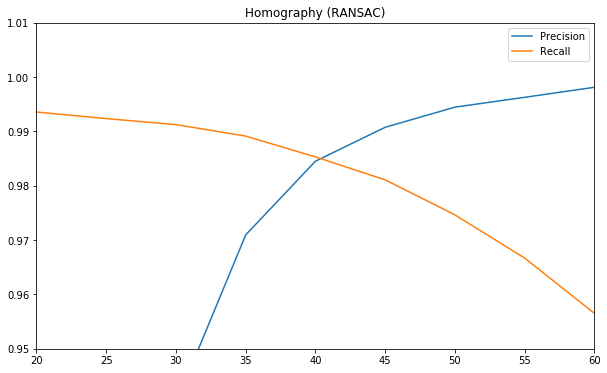
\includegraphics[width=\linewidth]{ransac-performance.png}
%     \caption[RANSAC performance]{Precision and recall, by threshold on the number of keypoints. This is but a small part from the whole curve, just showing values above $0.95$. The recall is always on an excellent level while the threshold should not be too low because precision will collapse otherwise.}
%     \label{fig:ransac}
% \end{figure}

% Using RANSAC leads to outstanding results. Values for precision and recall---depending on the threshold set for the number of keypoints---are close to their maximum of $1.0$. Moreover, the performance is much more robust concerning this threshold. See figure~\ref{fig:ransac} where even for larger thresholds the recall is always above $0.95$. These results come at a cost: a computational one. Calculating RANSAC is much more expensive in this regard than just matching keypoints. Of course, first filtering the keypoints before running RANSAC is an option for speeding up the computation, but too aggressive filtering will go at the expense of robustness. After some experiments, a maximum distiance between keypoints of $100$ was chosen.

% \begin{figure}
%     \centering
%     \begin{subfigure}{.49\textwidth}
%         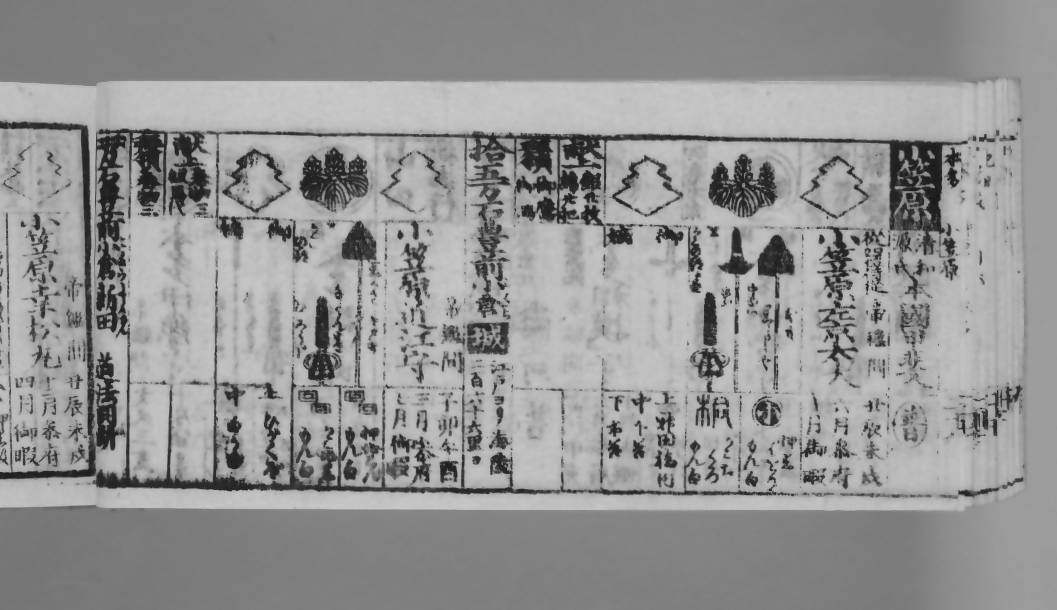
\includegraphics[width=\textwidth]{homography-good.jpg}
%         \caption{}
%     \end{subfigure}
%     \begin{subfigure}{.49\textwidth}
%         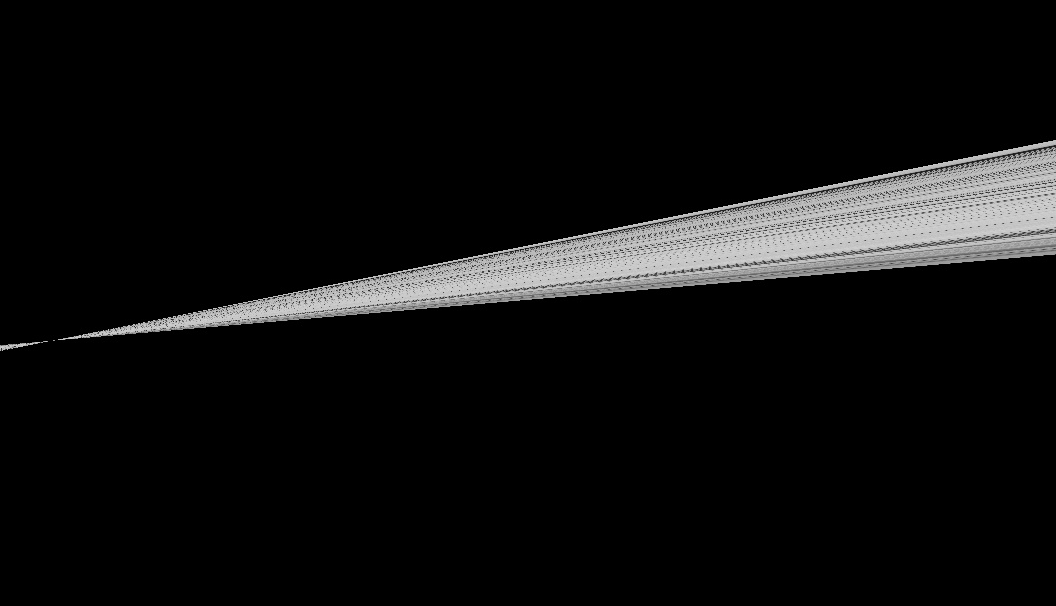
\includegraphics[width=\textwidth]{homography-bad.png}
%         \caption{}
%     \end{subfigure}
%     \begin{subfigure}{\textwidth}
%         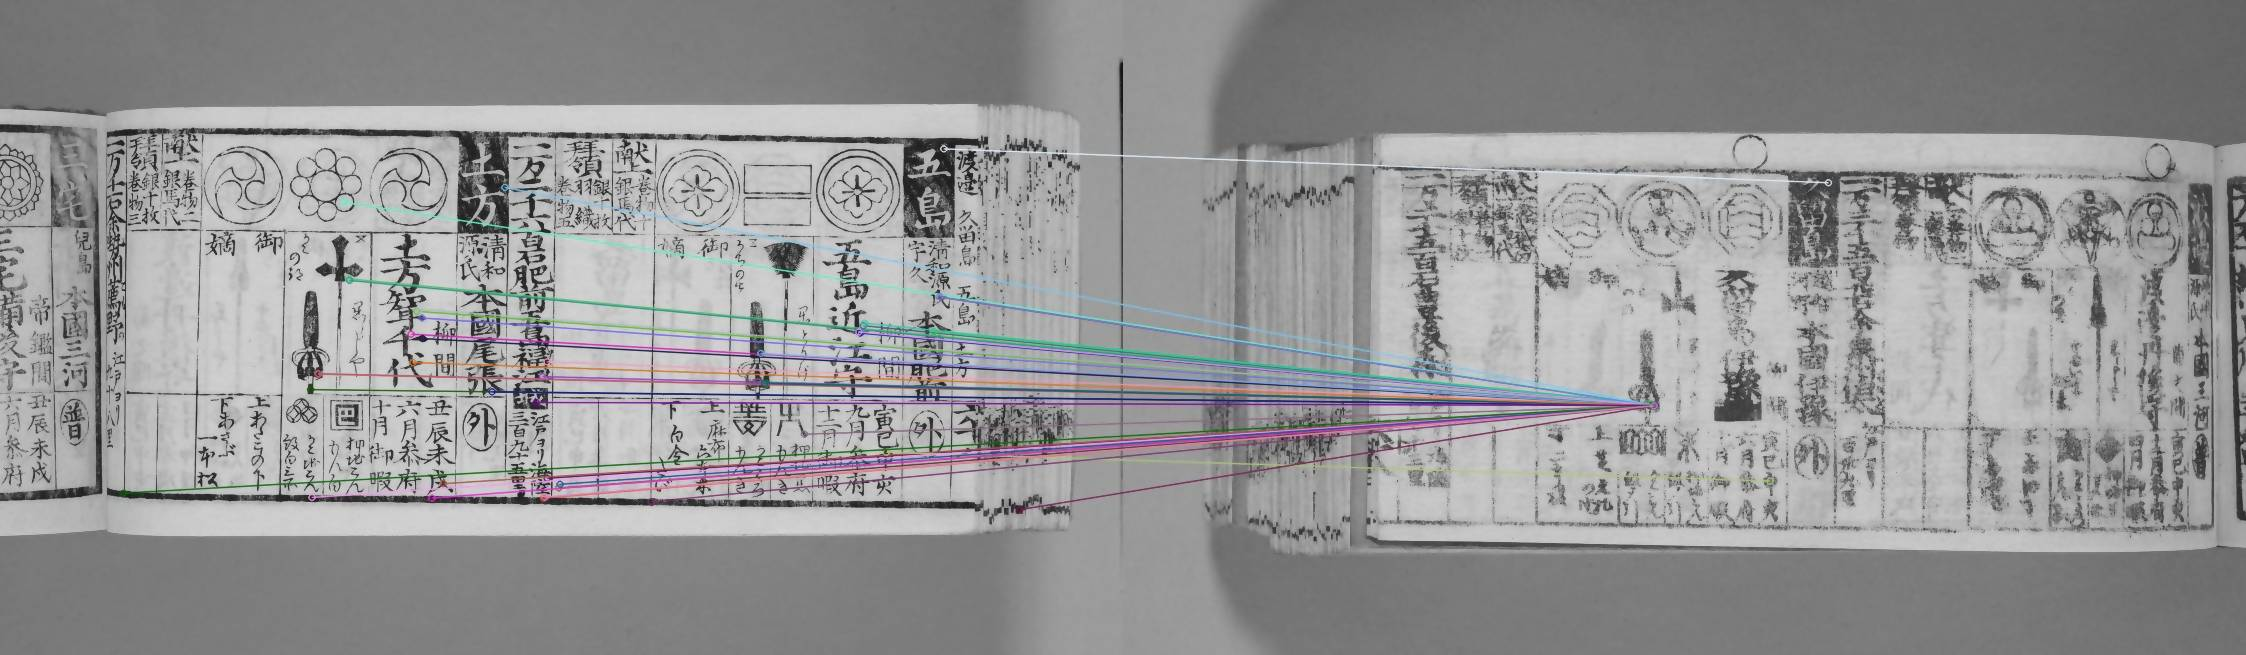
\includegraphics[width=\textwidth]{homography-cause.jpg}
%         \caption{}
%     \end{subfigure}
%     \caption[Projective transformation examples]{Two examples for projective transformations: In this case, a good transformation as in (a) will have no perceptible effect, just slightly shifting some pixels. The image in (b) is the result of a bad transformation, shifting perspective in a way the original image can not be recognized anymore. This is caused by incorrect keypoint matching as seen in (c) where the majority of keypoints on the left page is matched to a single point on the right page.}
%     \label{fig:homography-compare}
% \end{figure}

% A last source of failure that can easily be eliminated are extreme transformations in perspective as seen in figure~\ref{fig:homography-compare}. Caused by incorrect keypoint matching, RANSAC mistakenly results in extreme perspective shifts that nevertheless are deemed possible by the algorithm. This makes up for less than $1\%$ of false positives, but can be corrected by removing matches where the projective elements from $\mathbf{H}$ are too extreme. Accordingly, transformations must conform to these two inequalities:

% \begin{gather*}
%     |\mathbf{H}_{1,3}| \leq 0.001\\
%     |\mathbf{H}_{2,3}| \leq 0.001
% \end{gather*}

\section{Conclusion}

Lorem ipsum dolor sit amet, consectetur adipiscing elit. Quisque vehicula vitae ligula vitae pellentesque. Aliquam placerat commodo urna ac luctus. Nullam aliquam purus diam, vel ornare quam tempor at. In ut est tempus, finibus dolor sed, semper tortor. Cras pharetra mollis nisl. Praesent a nisl tellus. In faucibus, ipsum sit amet varius porta, leo nibh ultrices nisl, a porta nunc nisi commodo tortor. Aenean efficitur viverra urna. Mauris scelerisque orci faucibus, gravida neque non, rutrum enim.

Lorem ipsum dolor sit amet, consectetur adipiscing elit. Praesent neque ex, ultricies vulputate magna eu, dignissim consequat ligula. Etiam faucibus bibendum dolor, at ultricies. 

% The threshold of $0.001$ is quite conservative and might even be chosen one magnitude lower without much difference.

% \begin{figure}
%     \centering
%     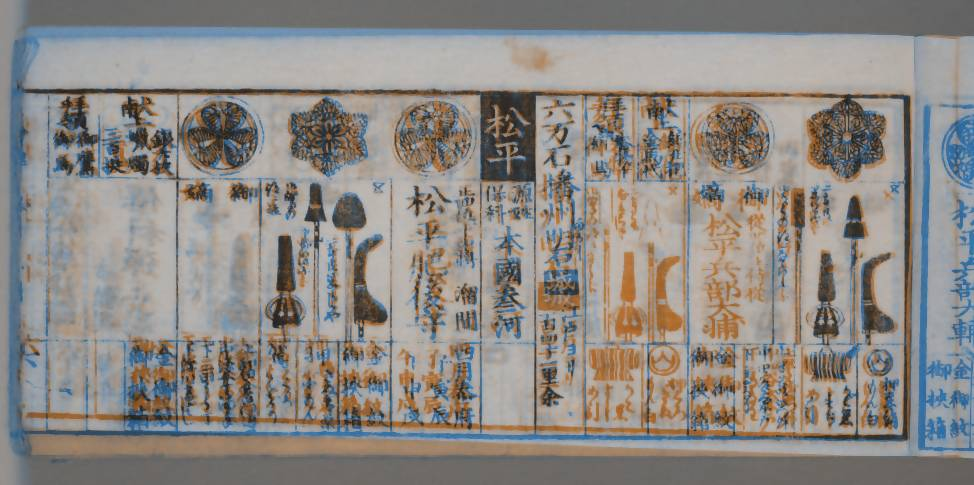
\includegraphics[width=\textwidth]{page-compare.jpg}
%     \caption[Visualizing page differences]{Visualizing page differences between two prints of the Shūchin Bukan (袖珍武鑑); page~13 from 1840 and page~15 from 1837. Differences are indicated by \textcolor{blue}{blueish} and \textcolor{red}{reddish} coloring respectively.}
%     \label{fig:page-compare}
% \end{figure}

% At the end of this work, there is a database holding information about matching keypoints and page transformations. For each matching page pair found, it is now possible to align them and applying simple, pixelwise operations for visualizing the differences. For an example see figure~\ref{fig:page-compare}.

% A scholar in the humanities and literature can now interactively browse these books and quickly identify interesting parts. This will hopefully lessen her burden when examining numerous pages, since small, abstract differences are often hard to discern for the human eye. So instead of exhausting her cognitive ability by staring at pages alone, it will now hopefully be easier to extract information from the actual content.

\printbibliography

\end{document}
